\section{Trends} \label{trends}

The challenges faced in the 2000s were the focus of the research that followed. Solutions to many of the challenges mentioned in Section~\ref{past} were proposed and major advancements were accomplished. In this section, we highlight some of the \emph{recent} trends in the area of software defect prediction. \revised{Furthermore, we discuss the game changers that pursed the accomplishments and had a significant impact on software defect prediction.}
Similar to the previous sections, we organize the trends along the four dimensions, data, metrics, models and performance evaluation.

%%%%%%%%%%%%%%%%%%%%%%%%%%%%%%%%%%%%%%%%%%%%%%%%%%%%%%%%%%%
\subsection{Data}

\smallsection{Trend 1: Availability and Openness}
Once the software defect prediction community realizes that data availability and openness is a key factor to its success, many defect prediction studies started sharing not only their data, but even their analysis scripts. For example, in 2004, NASA MDP (metrics data program) shared 14 datasets that are measured during the software development of NASA projects through the PROMISE repository (we will discuss the PROMISE repository later in this section)~\cite{promiserepo}. The NASA datasets were some of the first public datasets from industrial software projects to be shared in the defect prediction domain. Similarly, Zimmermann \ea ~\cite{Zimmermann2007}, D'Ambros \ea ~\cite{Dambros10MSR}, Jureczko \ea ~\cite{Jureczko2010PROMISE}, Kamei \ea ~\cite{kamei2013tse} and many others shared their open source data. In fact, many conferences now have special tracks to facilitate the sharing of datasets and artifacts. For example, the ESEC/FSE conference~\cite{FSE2015} now has a replication package track that encourages authors to share their artifacts. The MSR conference now has a dedicated data showcase track that focuses on the sharing of datasets that can be useful for the rest of the community.

Reflecting back, the recent trend of data sharing and openness have in many ways helped alleviate the challenge that existed in the early 2000s. That said, not all data is being shared; our community needs to continue to nourish such efforts in order to make data availability and openness a non-existing issue. 

%share the datasets that they collect from 3 versions of the Eclipse project. In 2010, share the datasets collected from 48 releases of 15 open source projects. provide the datasets measured from more than 450 versions of 5 open source software. The datasets include not only product metrics but also process metrics. In 2013,  share their change-level datasets that are collected from 6 open source software projects.


%There are only a part of papers that open their datasets.
%We believe that defect prediction studies are solving the problem in 2000 (i.e., software defect prediction studies was the lack of availability and openness of datasets).
% \emad{I am not sure what this is trying to say.}
% \yasu{The paragraph is "Reflecting back" is what I wanted to to say}


\smallsection{Trend 2: Types of Repositories}
In addition to using the traditional repositories such as bug and code repositories, recent studies have also explored other types of repositories. For example, Meneely and Williams~\cite{Meneely2010ESEM} leveraged the vulnerabilities database to examine the effect of the ``too many cooks in the kitchen'' phenomena on software security vulnerabilities. Other studies such as the study by Lee \ea ~\cite{Lee2011FSE} leveraged Mylyn repositories, which capture developer interaction events. McIntosh \ea ~\cite{McIntosh2014MSR} leveraged Gerrit data, which facilitate a traceable code review process for git-based software projects to study of the impact of modern code review practices on software quality. Other types of repositories are also being used, especially as software development teams become more appreciative of the power of data analytics.

Reflecting back, the recent trends show strong growth in the different types of repositories being used. We believe that exploring new repositories will have a significant impact on the future of software defect prediction since it will facilitate better and more effective models and allow us to explore the impact of different types of phenomena on software quality.
%\emad{Need to edit this}.



% such as selecting and editing software source, to extract and use 56 developer interaction metrics (e.g., the effort spent on a file).
%They show that the interaction metrics can outperform or improve defect prediction performance over using code or history metrics, improving F-measure by 0.2.


%They perform their case study on three open source systems (i.e., Linux kernel, PHP and Wireshark). They find that files changed by six developers or more were at least four times more likely to have a vulnerability than files changed by less than six developers.

%Through a case study of 3 open source projects, they find that code review coverage, participation, and expertise sh

% now we also use email, software inspection, testing.

\smallsection{Trend 3: Variety of Granularity}
Due to the benefits of performing predictions at a finer granularity, recent defect prediction studies have focused on more fine-grained level, such as the method level~\cite{Kim2007ICSE,Hata2012ICSE,Giger2012EMSE} and change level~\cite{Aversano2007,Kim2008TSE,kamei2013tse}. For example, Giger \ea ~\cite{Giger2012EMSE} empirically investigate whether or not defect prediction models at the \emph{method-level} works well. Another example of work that aims to perform predictions at a finer granularity is the work on change-level prediction, which aims to predict defect introducing changes (a.k.a commits). The advantage of predicting defect introducing changes, compared to subsystems or files is that a change is much smaller, can be easily assigned and contains complete information about a single change (which is important if a fix spans multiple files for example).

%The experimental results using 21 open source projects show that their prediction models can predict 88\% of defects with precision of 84\%.  
%For example of the change level, Kim \ea ~\cite{Kim2008TSE} use metrics extracted from source code changes to predict whether a change will be buggy (i.e., introduce a defect) or clean.
%They show that they can classify changes with an accuracy of 78\% and achieve an average of 60\% recall of buggy changes.

% now we also use change-level and method-level too.

\revised{
Reflecting back, the recent trends have realized that the practical value of the predictions decrease as the abstraction level increases (i.e., since more code would need to be inspected at high levels of abstraction). The recent trends show that they focus more on performing predictions at a finer level of granularity, e.g., at the method-level and change-level. 
}

\begin{oframed}
%\begin{leftbar}
\vspace{-0.2cm}
\smallsection{Game Changer 1: OSS projects} 
Open Source Initiative, which was founded in 1998 and is an organization to dedicate to promoting open source software, describes \emph{open source software is software that can be freely used, changed, and shared (in modified or unmodified form) by anyone.}~\cite{OSI}
Nowadays, there are no end of active open source software projects online supported by a huge range of people.

An OSS project is a change changer, because it opens the development history of long-lived widely-deployed software systems.
Figure \ref{fig:oss} shows that the number of papers using OSS projects is growing over time~\cite{Shihab2012PhD}. 

Other way to access such rich data source is to cooperate with commercial organization (e.g., ABB Inc,~\cite{Li2006} and Avaya~\cite{Mockus2010FSE}).
However, commercial organization in many cases is not willing to give access to the detail of its rich data source due to confidential reasons.
While another way is to use academic projects (e.g., course projects), such projects are relatively not rich comparing with commercial projects.
In short, OSS projects provide rich, extensive, and readily available software repositories. 
\end{oframed}

%-----------------------------------------------------------------------
\begin{figure}
  \centering
  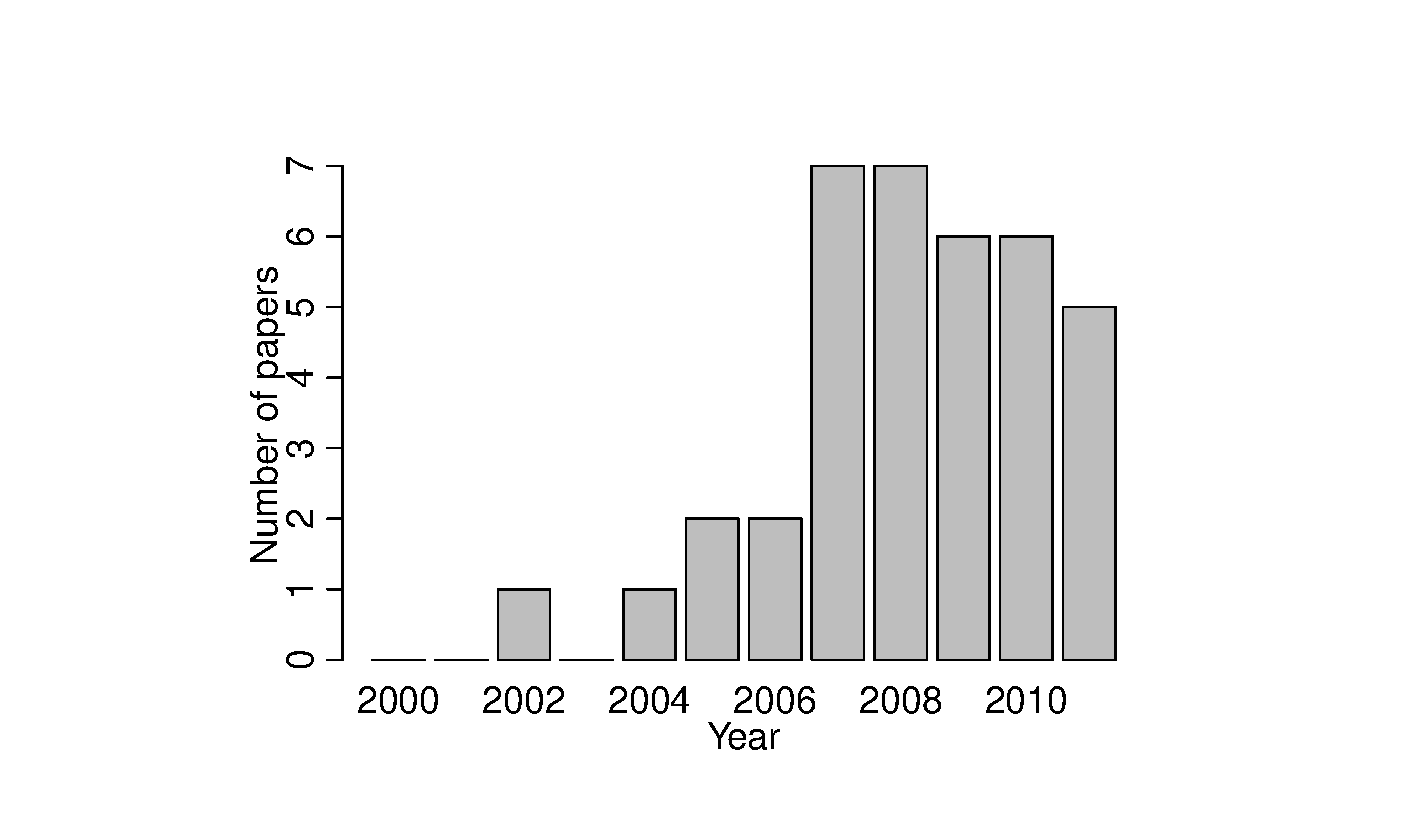
\includegraphics[trim=100 30 100 0, scale=0.5,clip]{figures/papers}
  \caption{The number of defect prediction papers using open source projects \label{fig:oss}}
\end{figure}
%-----------------------------------------------------------------------


\begin{oframed}
%\begin{leftbar}
\vspace{-0.2cm}
\smallsection{Game Changer 2: The PROMISE repository}
The PROMISE repository is a research data repository for software engineering research datasets and offers free and long-term storage for our research datasets~\cite{promiserepo}.
We can find more than 45 datasets about defect prediction in the PROMISE repository.
The PROMISE repository starts to share the samples of the Metrics Data Program, which was run by NASA for collecting static code measures in 2002, as version 1 in 2004.
The PROMISE repository is currently version 4 from 2014 and is upgraded to terabyte size.

The PROMISE repository is a game changer, because we can skip our own data collection processes and obtain promptly pre-processed and valuable datasets.
This dramatically speeds up the progress of defect prediction studies. 
The repository is in widespread use. For example, as of 2010, there are 73 papers that use the repository on IEEE Explorer~\cite{promiserepo}.
\end{oframed}

%%%%%%%%%%%%%%%%%%%%%%%%%%%%%%%%%%%%%%%%%%%%%%%%%%%%%%%%%%%
\subsection{Metrics}

\smallsection{Trend 4: Variety of Independent Variables}
In addition to using code metrics, recent software defect prediction used process metrics, which measure the change activity that occurred during the development of a new release, to build highly accurate defect prediction models~\cite{NagappanICSE05_2,Moser2008ICSE}. The idea behind using process metrics in defect prediction is that the process used to develop the code may lead to defects, hence the process metrics may be a good indicator of defects. For example, if a piece of code is changed many times or by many people, this may indicate that it is more likely to be defect prone.

Although much of the current research used process metrics to predict defects, other metrics have been proposed in the literature. For example, studies explored design/UML metrics~\cite{Briand2002TSE, Erika2010ICSE, Nugroho2010MSR} (which capture the design of the software system), social metrics~\cite{Bird2009ISSRE} (which combine dependency data from the code and from the contributions of developers), organizational metrics~\cite{Mockus2010FSE} (which capture the geographic distribution of the development organization, e.g., the number of sites that modified a software artifact) and ownership metrics~\cite{Bird2011FSE} (which measure the level of ownership of a developer to a software artifact.

%\revised{
%Reflecting back, the recent trends show the impact of not only code based metrics, but also a lot of variety of independent variables on software defects. We believe that exploring new metrics will be worth to the future of software defect prediction since defect prediction models need to capture the characteristics of the defects that our new environments raise (e.g., smart phones).
%}

Reflecting back, we saw a very clear evolution in the way software defect prediction work uses metrics. Initially, most metrics were deigned to help improve the prediction accuracy. However, more recently, studies have used defect prediction to examine the impact of certain phenomena, e.g., ownership, on code quality. Such studies have pushed the envelope in metric design and contributed significantly to the body of empirical work on software quality in general.
%\emad{I suggest we refactor what you revised to what I wrote here.}
% now we use process, social, experience as metrics.

\smallsection{Trend 5: Variety of Dependent Variables}
In the early 2000s, most studies used post-release defects as a dependent variable~\cite{Briand2002TSE,Denaro2002ICSE}. More recently however, many studies started to focus on different types of dependent variables that span much more than post-release defects. For example, Shihab \ea ~\cite{Shihab2011FSE} focused on predicting defects that break pre-existing functionality (breakage defects) and defects in files that had relatively few pre-release changes (surprise defects). Meneely and Williams~\cite{Meneely2010ESEM} built models to predict software security vulnerabilities. Garcia \ea~\cite{Garcia2014MSR} predicted blocking defects, which block other defects from being fixed. 
\revised{Furthermore, researchers have proposed to perform predictions at the change-level, focusing on predicting defect-inducing changes~\cite{Kim2008TSE, Mockus2000BTJ}. The prediction can be conducted at the time when the change is submitted for unit test (private view) or integration. Such immediate feedback ensures that the design decisions are still fresh in the minds of developers~\cite{kamei2013tse}.}

%\emad{should we discuss some of the change-level prediction stuff here?}

%and Chen \ea~\cite{Chen2014MSR} conduct an empirical study of dormant defects, which are introduced in a version of the software system, but are not found until much later.

Reflecting back, it seems that many of the recent studies have realized that not all defects are equal and that there are important defects that are not post-release defects. The recent trends show that different types of dependent variables are being considered, which take into account different stakeholders \revised{different timing}. For example, the prediction of blocking defects clearly shows that helping the developers in the main goal, which is different from the traditional defect prediction studies which mainly focused on the customer as the main stakeholder. \revised{The prediction of defect-inducing changes shows that predictions are made early on, comparing with the traditional studies which have their drawbacks (i.e., predictions are made too late in the development cycle).}

%\emad{should we discuss some of the change-level prediction stuff here?}

\begin{oframed}
%\begin{leftbar}
\vspace{-0.2cm}
\smallsection{Game Changer 3: SZZ algorithm}
\'{S}liwerski \ea ~proposed the SZZ algorithm\footnote{SZZ stands for the capital letter of authors' last name, \'{S}liwerski, Zimmermann and Zeller.}~\cite{sliwerski2005} that extracts whether or not a change introduces a defect from VCSs. The SZZ algorithm links each defect fix to the source code change introducing the original defect by combining information from the version archive (such as CVS) with the bug tracking system (such as Bugzilla).

The SZZ algorithm is a game changer, because it provides new data source for defect prediction studies. Without the SZZ algorithm, we can rarely access the information about when a change induces a defect and conduct empirical studies on defect prediction models.
When developers submit their revision for adding functionality and modifying defects to VCSs in their project, they enter their comments (e..g, fix bug \#1000) related to their revision in log messages.
However, there is no comments to detect that a change induces a defect (e.g., introducing defects), because developers 
have no intention of introducing defects and introduce them wrongly.
Therefore, before SZZ algorithm was proposed, it is difficult to automatically recover new data source (i.e., change-level bug information). 

Today (September 2015), the paper~\cite{sliwerski2005} is cited by more than 400 papers according to Google Scholar\footnote{\url{https://goo.gl/lUiGbR}}. The algorithm is not only used for making dataset, but also opens to a new research topic (e.g., improving the accuracy of the algorithm~\cite{Kim2006ASE}).
\end{oframed}
%\end{leftbar}

%%%%%%%%%%%%%%%%%%%%%%%%%%%%%%%%%%%%%%%%%%%%%%%%%%%%%%%%%%%
\subsection{Model building}
\smallsection{Trend 6: Treating Uncertainty in Model Inputs or Outputs}
%\emad{Yasu, we need to explain what the issue is here....you go directly into ensemble learning, but it is not clear why. We should start by giving some background and highlight the problem first man.}
As we mentioned in Section \ref{past}, defect prediction models assume that the distributions of the metrics in the training and testing datasets are similar~\cite{Turhan2009ESE}. However, in practice, the distribution of metrics can vary among releases. 
To treat with projects that did not have the similar distributions of the metrics between training and testing datasets, recent defect prediction studies have used ensemble techniques.
One of the frequently-used ensemble techniques is random forests classifiers that consist of a number of tree-structured classifiers~\cite{Guo2004ISSRE,mende2009,Kamei2010ICSM}. New objects are classified from an input vector that is composed of input vectors on each tree in the forest. Each tree casts a vote at the input vector by providing a classification. The forest selects the classification that has the most votes over all trees in the forest.

The main advantages of random forest classifiers are that they generally outperform simple decision trees algorithms in terms of prediction accuracy. Also, random forest classifiers are more resistant to noise in data~\cite{Marks2011PROMISE}.

Reflecting back, the recent trends of using ensemble techniques (e.g., random forests) migrates the problem that, if the distribution of metrics vary among releases, simple modeling techniques fail prediction due to specializing only in training data.

%\smallsection{Building Models for Projects in the Initial Development Phases}
\smallsection{Trend 7: Building Cross-Project Defect Prediction Models for Projects in the Initial Development Phases}
%\emad{I think we should rename this section to cross-project defect prediction since that is what it is really about.}
%\yasu{I agree}
The majority of studies in the early 2000s focused on within-project defect prediction. This means that they used data from the same project to build their prediction models. However, one major drawback with such an approach that was recently highlighted is the fact that within-project defect prediction requires sufficient historical data, for example, data from past releases. The requirement of historical data can be a challenge, especially for newer projects. Hence, more recently, defect prediction studies have worked on cross-project defect prediction models, i.e., models trained using historical data from other projects~\cite{Menzies2013TSE, Nam2013ICSE, Turhan2009ESE, Zhang2014MSR, Zimmermann2009FSE}, in order to make defect prediction models available for projects in the initial development phases, or for legacy systems that have not archived historical data. For example Briand \ea ~\cite{Briand2002TSE} train a defect prediction model using data from one system, and test it using data from another system.

At the beginning of cross-project defect prediction models, they show that the prediction performance for the cross-project context is lower than the within-project one. However, later on, recent work has shown that cross-project models can achieve performance similar to that of within-project models. For example, in their award wining work, Zhang \ea ~\cite{Zhang2014MSR} proposes a context-aware rank transformation method to preprocess predictors, address the variations in their distributions and showed that their cross-project models achieve performance that rivals within-project models.

Reflecting back, thanks to cross-project defect prediction models, the recent defect prediction models are now available for the projects in the initial development phases or for legacy systems that have not archived historical data.
At this point, the research community has come a long way with cross-project defect prediction, however, many questions still remain. For example, the lack of availability of industrial data leaves open the question of whether models built using data from open source projects would apply to industrial projects. At this stage, cross-project defect prediction remains as an open research area.
% \emad{should we discuss some of the change-level prediction stuff here?}
% \yasu{Already we discuss change-level prediction stuff. So I don't think we should discuss.}

\begin{oframed}
%\begin{leftbar}
\vspace{-0.2cm}
\smallsection{Game Changer 4: Weka and R}
The majority of defect prediction studies use WEKA or R. WEKA~\cite{WEKA} is a tool developed by the Machine Learning Group at University of Waikato. Weka is a collection of machine learning algorithms for data mining tasks that can be applied directly to a dataset. Another commonly used tool in defect prediction studies is R~\cite{R}. R is an open source language and environment for statistical analysis.

Weka and R are game changers, because both of them provide a wide variety of data pre-processing, statistical (linear and nonlinear modelling, classical statistical tests and classification) and support for graphical techniques. They also are open source software and highly extensible. Therefore, Weka and R are commonly used in defect prediction studies. In fact, 21\% and 8\% of the papers published in defect prediction studies between 2003 and 2011 used Weka and R as tools~\cite{Shihab2012PhD}. 
\end{oframed}

% we now also work on cross-projects.

%%%%%%%%%%%%%%%%%%%%%%%%%%%%%%%%%%%%%%%%%%%%%%%%%%%%%%%%%%%
\subsection{Model evaluation}

\smallsection{Trend 8: Practical Performance Measures}
In the early 2000s, most studies used traditional performance evaluation techniques such as precision and recall. More recently defect prediction studies have focused on more practical performance evaluations. To consider evaluation in more practical setting, recent work has considered the effort required to address the predicted software artifacts~\cite{Kamei2010ICSM, Mende2010CSMR, Menzies2010ESE}. 
For example, recent work by Kamei \ea ~\cite{Kamei2010ICSM} evaluates common defect prediction findings (e.g., process metrics vs. product metrics and package-level prediction vs. file-level prediction) when effort is considered. 
%Mende and Koschke~\cite{Mende2010CSMR} compare two strategies to include the effort treatment into defect prediction models.
%One strategy is applicable to any probabilistic classifier and the other applicable only for regression algorithms.
Mende and Koschke~\cite{Mende2010CSMR} compared strategies to include the effort treatment into defect prediction models.
Menzies \ea ~\cite{Menzies2010ESE} argue that recent studies have not been able to improve defect prediction results since their performance is measured as a tradeoff between the probability of false alarms and probability of detection. Therefore, they suggest changing the standard goal to consider effort, i.e., to finding the smallest set of modules that contain most of the errors.

Furthermore, recent defect prediction studies have also conducted an interview to better understand the defect prediction models and derive practical guidelines for developing high quality software. For example, Shihab \ea ~\cite{Shihab2011FSE} ask the opinions of the highly experienced quality manager in the project about their prediction results. Based on their opinions, the authors conclude that the defect prediction models should not only predict defect locations, but also detect patterns of changes that are suggestive of a particular type of defect and recommend appropriate remedies. 

%Bird \ea ~\cite{Bird2011FSE}  disucsed  with engineers at Microsoft based on their observation of the relationship between ownership measures and software defects.  Tan \ea ~\cite{Tan2015ICSE} have interaction with developers and identify some directions such as showing the prediction  precision on historical data.

Reflecting back, we see that more recent studies have focused on the practical value of software defect prediction and try to evaluate their models in realistic settings. We strongly support such research and see this trend continuing to grow since software defect prediction models are starting to be used in industry (e.g.,~\cite{Shihab2011FSE}).


\smallsection{Trend 9: Transparency/Repeatability}
As mentioned earlier, the software engineering community as a whole has realized the value of making studies as transparent as possible. For example, recent defect prediction studies have kept transparency for their studies, then generated a  a lively discussion (e.g., critique) of the results of the studies and led to new findings.
For example, Shepperd \ea \cite{Shepperd2013TSE} derive some comments on the NASA software defect datasets (e.g., the dataset contains several erroneous and implausible entries) and share cleaned NASA defect datasets. Then, Ghotra \ea ~\cite{Ghotra2015ICSE} revisit the findings of Lessmann \ea ~\cite{Lessmann2008TSE} that used original NASA datasets. In contrary to prior results~\cite{Lessmann2008TSE}, Ghotra \ea ~shows that there are statistically significant differences in the performance of defect prediction models that are trained using different classification techniques. Such valuable are made possible thanks to the fact that the NASA projects made their datasets available.  

\begin{comment}
\emad{I don't get how the paragraph fits/relates to this section} 
\yasu{I agree. I commented out the paragraph now.}
Furthermore, defect prediction studies are likely to lead to extension studies by sharing the datasets and scripts that the studies use in their experiment.  For example, Zimmermann \ea ~\cite{Zimmermann2007} collect the datasets including product metrics from 3 versions of the Eclipse project, conduct an empirical study on defect prediction models using their own datasets and share the datasets in their web site.
Then, Moser \ea ~\cite{Moser2008ICSE} perform a comparative analysis of the efficiency of process metrics and product metrics for defect prediction by extending the datasets (i.e., only collecting process metrics) Zimmermann \ea ~\cite{Zimmermann2007} shared.
\end{comment}

Reflecting back, we see a very healthy and progressive trend where software defect prediction studies are becoming more transparent. Such changes will only make our findings more practical and will encourage use to advance the science (not only the engineering) behind the area of software defect prediction since it allows us to repeat and scrutinize assumptions of prior studies.

% Some paper shares their data and scripts to re-run their analysis.

% Sounds nice.
% Number of papers whose title contains the string "mobil" (accounting for both "mobile" and "mobility") published in flagship software engineering venues (TSE, TOSEM, ICSE, ASE, ESEC/FSE).

% http://ieeexplore.ieee.org/Xplorehelp/#/searchingIeeeXplore/usingAdvancedSearch/commandSearch/fieldCodes

